\documentclass{beamer}

\usetheme{Boadilla}
\usecolortheme{beaver}

\usepackage{graphicx}
\graphicspath{ {./images/} }

\title{Class Snap}
\subtitle{Student Showcase 2024}
\author{Logan Humbert}
\institute{Colorado Mesa University}
\date{April 26, 2024}
\titlegraphic{
\includegraphics[width=2cm]{cmu_logo}}

\begin{document}
	\frame{\titlepage}
	
	\begin{frame}
		\frametitle{Table of Contents}
		\tableofcontents
	\end{frame}
	
	\section{Introduction}
	\begin{frame}
		\frametitle{Introduction}
		
		\begin{alertblock}{Class Snap}
			Multi-platform application for students
			\linebreak
			- Take notes in class easily
			\linebreak
			- Review and modify them later
		\end{alertblock}
	\end{frame}
	
	\section{The problem}
	\begin{frame}
		\frametitle{The problem}
		
		\begin{alertblock}{Traditional Note-Taking}
			\begin{itemize}
				\item Disorganization: Messy notes leading to difficulty to find information
				\item Inefficiency: Time wasted organizing our notes
				\item Space waste: Lot of space needed to keep all notes
			\end{itemize}
		\end{alertblock}
		
		\begin{alertblock}{Other digital solutions}
			Pros:
			\begin{itemize}
				\item  Keep notes clean and structured (erase/rewrite, highlight information)
				\item Keep all notes in one location
				\item Easy to find a note or information in note
			\end{itemize}
			
			Cons:
			\begin{itemize}
				\item Many features -- time wasted to find them
				\item Great to use on a laptop, not really on a phone
			\end{itemize}
		\end{alertblock}
	\end{frame}
	
	\section{Requirements}
	\begin{frame}
		\frametitle{Requirements}
		
		\begin{alertblock}{Main goal}
			Help students taking notes easily for their different classes and organizing them by class
		\end{alertblock}
		
		\begin{alertblock}{User stories}
			A user must be able to:
			\begin{itemize}
				\item See his different classes
				\item Add/edit/ delete a class
				\item Create/edit/delete a note for any class he has created
				\item View a note
				\item  Search for a class or a note by name
			\end{itemize}
		\end{alertblock}
	\end{frame}
	
	\section{Iterative Design}
	\subsection{Designing/Prototyping}
	\begin{frame}
		\frametitle{Iterative Design}
		\framesubtitle{Designing/Prototyping}
		
		\begin{alertblock}{Figma}
			Tool for designing/prototyping applications
		\end{alertblock}
		
		\begin{figure}
			\centering
			\begin{minipage}{1\textwidth}
				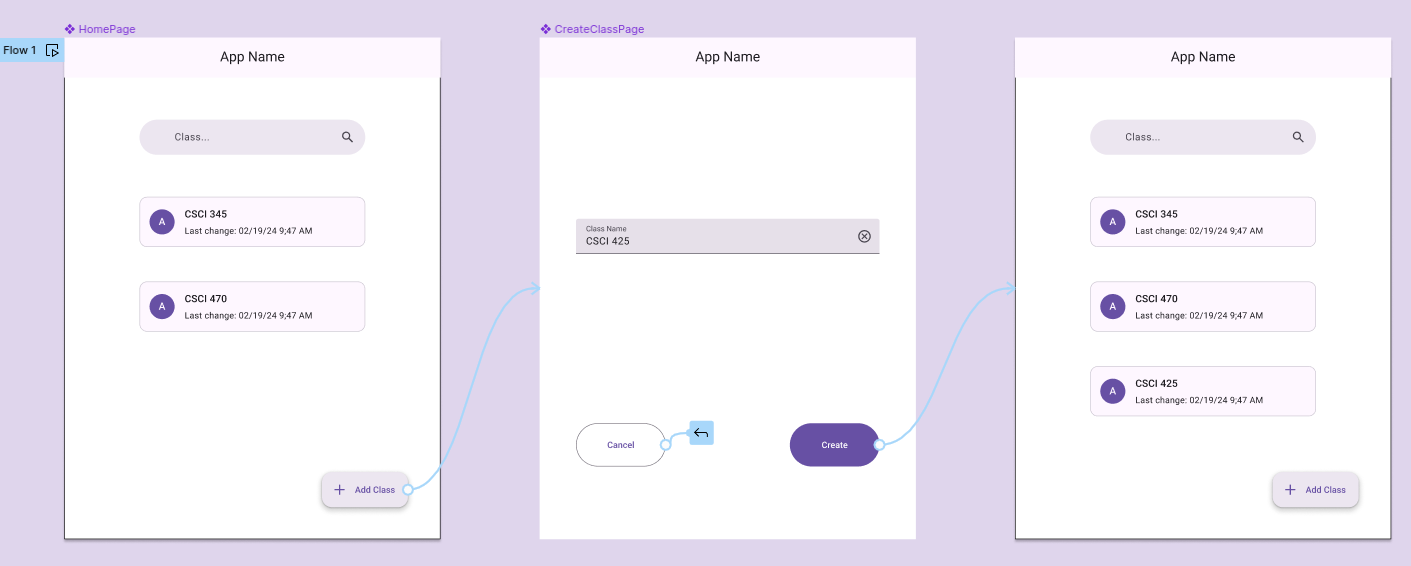
\includegraphics[width=\linewidth]{figma_user_story_create_class}
			\end{minipage}
		\end{figure}
	\end{frame}
	
	\subsection{Developing}
	\begin{frame}
		\frametitle{Iterative Design}
		\framesubtitle{Developing}
		
		\begin{alertblock}{Flutter}
			Framework made by Google
			\linebreak
			Create multi-platform apps
			\linebreak
			Uses dart as programming language
		\end{alertblock}
	\end{frame}
	
	\subsection{UI/UX tests}
	\begin{frame}
		\frametitle{Iterative Design}
		\framesubtitle{UI/UX tests}
		\begin{alertblock}{Objectives}
			Ask potential users to try the app and give feedback on the design and experience they had
			\linebreak
			- Fix design flaws
			\linebreak
			- Improve the user experience
		\end{alertblock}
	
		\begin{figure}
			\centering
			\begin{minipage}{0.16\textwidth}
				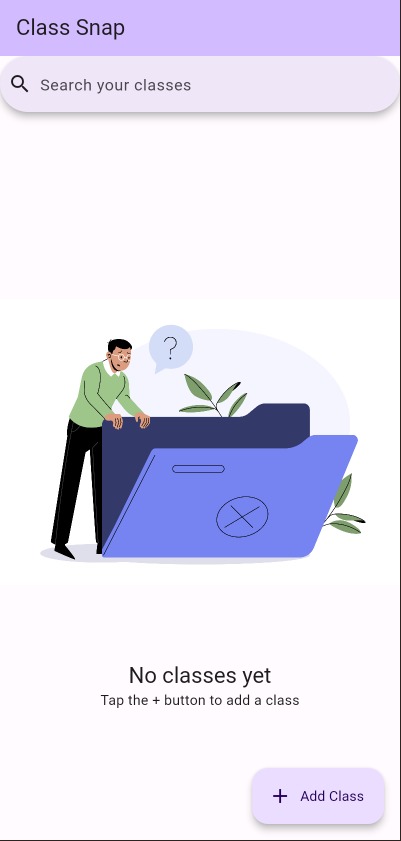
\includegraphics[width=\linewidth]{list_empty_fixed}
			\end{minipage}
			\hspace*{0.5cm} 
			\begin{minipage}{0.16\textwidth}
				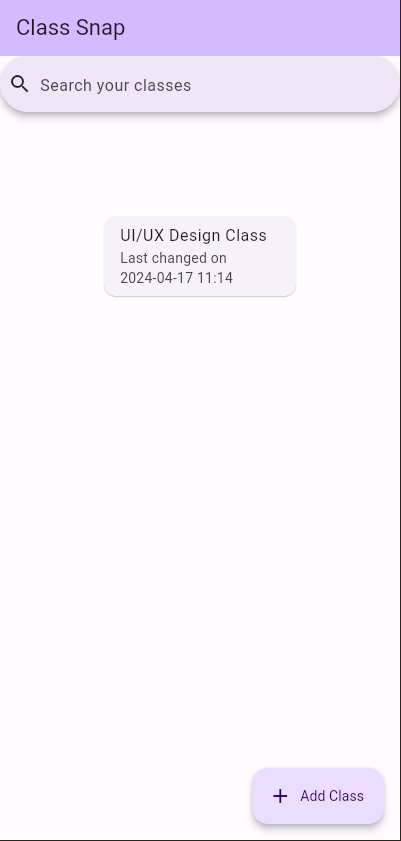
\includegraphics[width=\linewidth]{fix_bug_naming}
			\end{minipage}
		\end{figure}
	\end{frame}
	
	\subsection{Demo}
	\begin{frame}
		\frametitle{Iterative Design}
		\framesubtitle{Demo}
		
		\begin{alertblock}{Access the app}
			www.class-snap.tech
			
			\begin{figure}
				\centering
				\begin{minipage}{0.4\textwidth}
					
\includegraphics[width=\linewidth]{qrcode}
				\end{minipage}
			\end{figure}
		\end{alertblock}
	\end{frame}
	
	\section{Conclusion}
	\begin{frame}
		\frametitle{Conclusion}
		
		\begin{alertblock}{Objectives fulfilled?}
			Requirements correctly integrated in final product
		\end{alertblock}
		
		\begin{alertblock}{What is next?}
			\begin{itemize}
				\item Add more useful features (Adding hand-drawn notes)
				\item Add cloud storage
				\item Add support for exporting notes (pdf, word)
			\end{itemize}
		\end{alertblock}
	\end{frame}
	
	\begin{frame}
		\frametitle{The End}
		
		\centering
		Thank you for your attention!
		\linebreak
		Do you have any question?
	\end{frame}
\end{document}